%% LyX 2.2.0 created this file.  For more info, see http://www.lyx.org/.
%% Do not edit unless you really know what you are doing.
\documentclass[english]{beamer}
\usepackage[T1]{fontenc}
\usepackage[latin9]{inputenc}
\setcounter{secnumdepth}{3}
\setcounter{tocdepth}{3}
\usepackage{babel}
\usepackage{calc}
\usepackage{amstext}
\usepackage{graphicx}
\ifx\hypersetup\undefined
  \AtBeginDocument{%
    \hypersetup{unicode=true,pdfusetitle,
 bookmarks=true,bookmarksnumbered=false,bookmarksopen=false,
 breaklinks=false,pdfborder={0 0 1},backref=false,colorlinks=true}
  }
\else
  \hypersetup{unicode=true,pdfusetitle,
 bookmarks=true,bookmarksnumbered=false,bookmarksopen=false,
 breaklinks=false,pdfborder={0 0 1},backref=false,colorlinks=true}
\fi

\makeatletter

%%%%%%%%%%%%%%%%%%%%%%%%%%%%%% LyX specific LaTeX commands.
%% Because html converters don't know tabularnewline
\providecommand{\tabularnewline}{\\}

%%%%%%%%%%%%%%%%%%%%%%%%%%%%%% Textclass specific LaTeX commands.
 % this default might be overridden by plain title style
 \newcommand\makebeamertitle{\frame{\maketitle}}%
 % (ERT) argument for the TOC
 \AtBeginDocument{%
   \let\origtableofcontents=\tableofcontents
   \def\tableofcontents{\@ifnextchar[{\origtableofcontents}{\gobbletableofcontents}}
   \def\gobbletableofcontents#1{\origtableofcontents}
 }
 \newenvironment{lyxcode}
   {\par\begin{list}{}{
     \setlength{\rightmargin}{\leftmargin}
     \setlength{\listparindent}{0pt}% needed for AMS classes
     \raggedright
     \setlength{\itemsep}{0pt}
     \setlength{\parsep}{0pt}
     \normalfont\ttfamily}%
    \def\{{\char`\{}
    \def\}{\char`\}}
    \def\textasciitilde{\char`\~}
    \item[]}
   {\end{list}}

%%%%%%%%%%%%%%%%%%%%%%%%%%%%%% User specified LaTeX commands.
\usetheme[secheader]{Boadilla}
\usecolortheme{seahorse}
\title[Declarative Concurrency in Join Calculus]{Declarative Concurrent Programming with Join Calculus}
\author{Sergei Winitzki}
\date{October 16, 2017}
\institute[Workday, Inc.]{Scala Bay}

\makeatother

\begin{document}
\frame{\titlepage}
\begin{frame}{What is ``Join Calculus''?}

Join calculus is...
\begin{itemize}
\item a \emph{declarative language} for concurrent \& parallel computations
\item ...largely unknown and unused by the software engineering community 
\end{itemize}
\end{frame}

\begin{frame}{Concurrent \& parallel programming is hard}

Imperative concurrency is difficult to reason about:
\begin{itemize}
\item callbacks, threads, semaphores, mutex locks
\item errors with shared mutable state
\item testing is hard \textendash{} non-deterministic runtime behavior!
\begin{itemize}
\item race conditions, deadlocks, livelocks
\end{itemize}
\end{itemize}
We can avoid this if we use declarative approaches:
\begin{itemize}
\item synchronous parallelism (parallel collections, Spark)
\item asynchronous parallelism (\texttt{\textcolor{blue}{\scriptsize{}Future}},
\texttt{\textcolor{blue}{\scriptsize{}async}}/\texttt{\textcolor{blue}{\scriptsize{}await}})
\item asynchronous streaming (Akka Streaming)
\item STM
\item Actors (Akka)
\item join calculus (\href{https://github.com/Chymyst/chymyst-core}{Chymyst})
\end{itemize}
\end{frame}

\begin{frame}{``Dining philosophers''}


\framesubtitle{The paradigmatic example of concurrency}

\href{https://en.wikipedia.org/wiki/Dining_philosophers_problem}{Five philosophers sit at a round table},
taking turns eating and thinking for random time intervals
\begin{center}
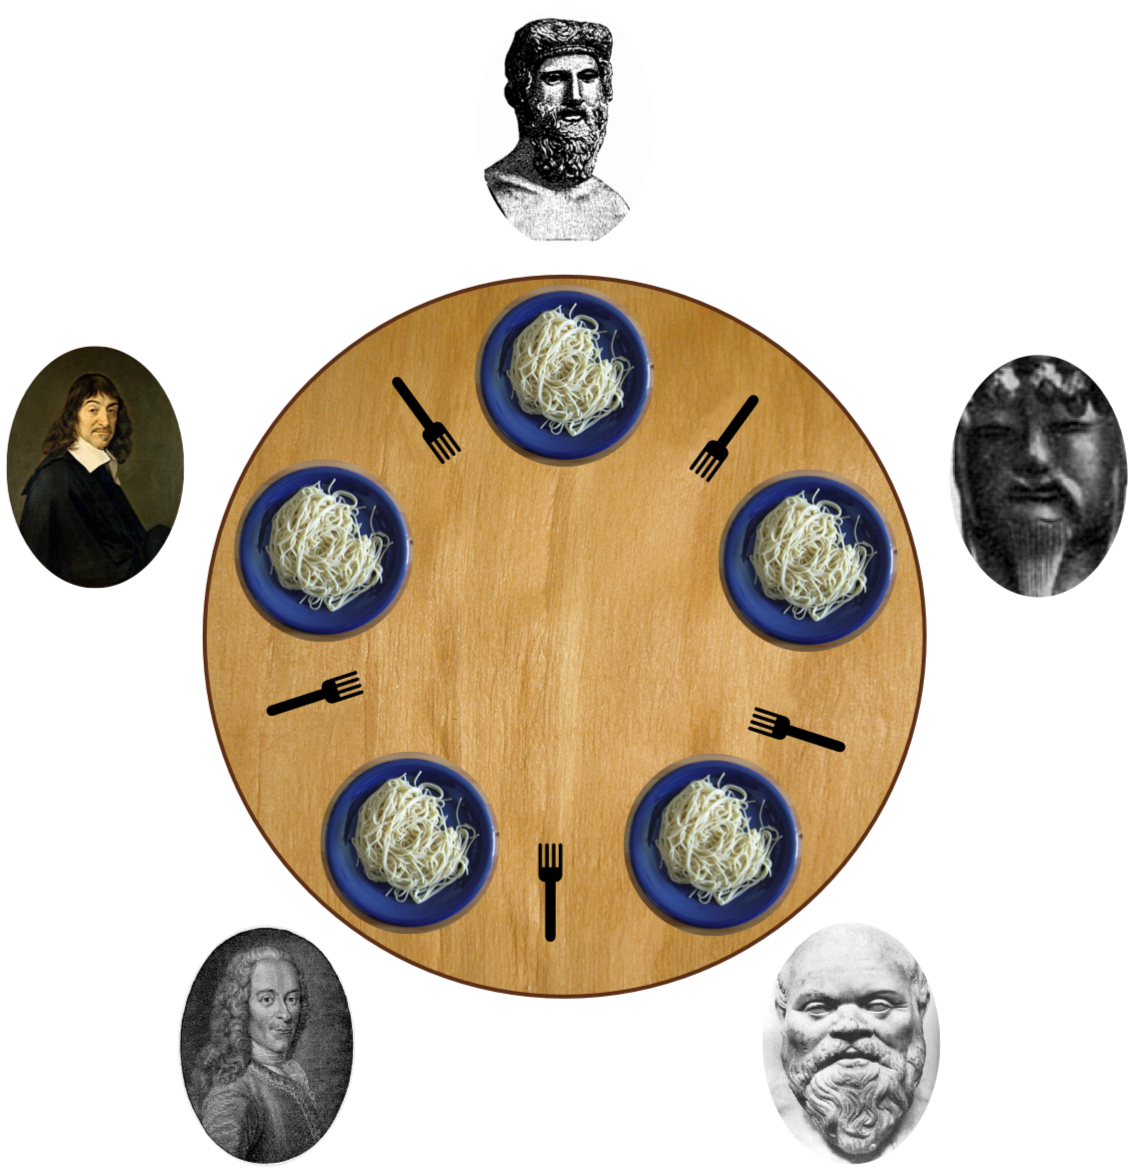
\includegraphics[height=4cm]{An_illustration_of_the_dining_philosophers_problem}
\par\end{center}

Problem: simulate the process, avoiding deadlock and starvation

Solutions: \href{https://rosettacode.org/wiki/Dining_philosophers}{Rosetta Code}
\end{frame}

\begin{frame}{Talk overview}


\framesubtitle{How I learned to forget semaphores and to love concurrency}

In this talk:
\begin{itemize}
\item Introduction to join calculus and ``chemical'' style of concurrency
\item \href{https://github.com/chymyst/chymyst-core}{Chymyst} -{}- a new
Scala EDSL for join calculus
\item Join calculus as an evolution of the Actor model
\item Examples and demos
\end{itemize}
Not in this talk: Other approaches to declarative concurrency
\begin{itemize}
\item $\pi$-calculus, PICT language (academic so far)
\item \texttt{Erlang's} message-passing $\approx$ Akka's ``Actors''
\item CSP / \texttt{Go} language
\item STM (Haskell)
\end{itemize}
\end{frame}

\begin{frame}{Join Calculus: A New Hope}


\framesubtitle{...and some new hype}

Join calculus is ...
\begin{itemize}
\item ...a declarative language for general-purpose concurrency
\item ``What if Actors were auto-started, type-safe, and multiple-dispatch''
\item No threads/semaphores/locks, no shared mutable state
\item Concurrency is automatic and \emph{data-driven}, not command-driven
\begin{itemize}
\item Easier to reason about than any other concurrency formalism!
\end{itemize}
\end{itemize}
Metaphors for join calculus:
\begin{itemize}
\item ``concurrent functions compute with concurrent data''
\item ``chemical soup with molecules and reactions'' 
\end{itemize}
\end{frame}

\begin{frame}{Concurrent data and concurrent functions}


\framesubtitle{Intuitions leading to join calculus}

What would it mean to make ordinary functions concurrent?
\begin{itemize}
\item Several functions should be able to run at once
\item No shared state: Concurrent processes work on different data
\end{itemize}
This will be implemented if:
\begin{itemize}
\item Data items and functions are stored in a special \textbf{site}
\item Each data item is labeled for specific concurrent function(s)
\item Concurrent functions consume data from the site
\item Computed results are emitted back to the site
\end{itemize}
Operational semantics:
\begin{itemize}
\item Concurrent functions auto-start whenever input data is available
\item Different instances of a concurrent function consume separate data
\end{itemize}
\end{frame}

\begin{frame}{Join Calculus: The Genesis}


\framesubtitle{a.k.a.~the ``Reflexive Chemical Abstract Machine'' {[}\href{http://citeseerx.ist.psu.edu/viewdoc/summary?doi=10.1.1.32.3078}{Fournet \&{} Gonthier 1996}{]}}

Real chemistry:
\[
\text{HCl}+\text{NaOH}\rightarrow\text{NaCl}+\text{H}_{2}\text{O}
\]

Abstract chemistry:
\begin{itemize}
\item The chemical ``soup'' contains arbitrarily defined ``molecules''
\item A combination of certain molecules starts a ``chemical reaction''
\end{itemize}
~\\

\fbox{\begin{minipage}[c][1\totalheight][t]{0.5\columnwidth}%
\begin{center}
``Abstract'' chemical laws:\\
\texttt{\textcolor{blue}{\footnotesize{}a + b ${\color{blue}\rightarrow}$
a}}\\
\texttt{\textcolor{blue}{\footnotesize{}a + c ${\color{blue}\rightarrow}$
$\textrm{�}$}}
\par\end{center}%
\end{minipage}}\hfill{}%
\begin{minipage}[c][1\totalheight][t]{0.3\columnwidth}%
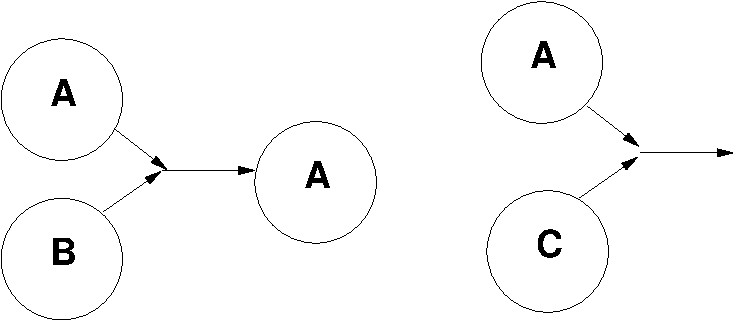
\includegraphics[width=1\columnwidth]{cham1a}%
\end{minipage}\hfill{}

~\\

\begin{itemize}
\item Program code defines molecules \texttt{\textcolor{blue}{\scriptsize{}a}},
\texttt{\textcolor{blue}{\scriptsize{}b}}, \texttt{\textcolor{blue}{\scriptsize{}c}},
... and arbitrary chemical laws
\item Emit some molecules into the ``soup''
\item The runtime system evolves the soup \emph{concurrently} and \emph{in
parallel}
\end{itemize}
\end{frame}

\begin{frame}{Join Calculus in a Nutshell}


\framesubtitle{``Better concurrency through chemistry''}

Translating the ``chemical metaphor'' into practice:~\\
~

\fbox{\begin{minipage}[c][1\totalheight][t]{0.5\columnwidth}%
\begin{itemize}
\item Each molecule carries a \textbf{value} (``concurrent data'')
\item Each reaction computes a ``molecule-set-valued'' expression from
input values
\item Resulting molecules are emitted back into the soup
\item Whenever input molecules are available, reactions start concurrently
and in parallel
\end{itemize}
%
\end{minipage}}\hfill{}%
\begin{minipage}[c][1\totalheight][t]{0.45\columnwidth}%
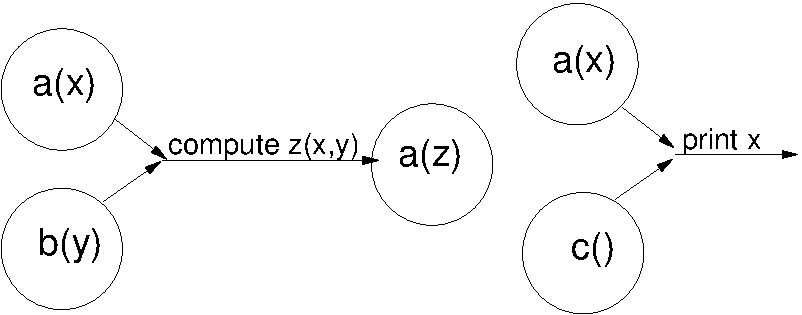
\includegraphics[width=1\columnwidth]{cham2}

~\\
\texttt{\textcolor{blue}{\scriptsize{}site(}}{\scriptsize \par}

\texttt{\textcolor{blue}{\scriptsize{}~ go \{ case }}\texttt{\textbf{\textcolor{blue}{\scriptsize{}a}}}\texttt{\textcolor{blue}{\scriptsize{}(x)
+ }}\texttt{\textbf{\textcolor{blue}{\scriptsize{}b}}}\texttt{\textcolor{blue}{\scriptsize{}(y)
$\Rightarrow$}}{\scriptsize \par}

\texttt{\textcolor{blue}{\scriptsize{}~ ~val z = f(x,y); }}\texttt{\textbf{\textcolor{blue}{\scriptsize{}a}}}\texttt{\textcolor{blue}{\scriptsize{}(z)
\},}}{\scriptsize \par}

\texttt{\textcolor{blue}{\scriptsize{}~ go \{ case }}\texttt{\textbf{\textcolor{blue}{\scriptsize{}a}}}\texttt{\textcolor{blue}{\scriptsize{}(x)
+ }}\texttt{\textbf{\textcolor{blue}{\scriptsize{}c}}}\texttt{\textcolor{blue}{\scriptsize{}(\_)
$\Rightarrow$}}{\scriptsize \par}

\texttt{\textcolor{blue}{\scriptsize{}~ ~ ~ println(x) \}}}{\scriptsize \par}

\texttt{\textcolor{blue}{\scriptsize{})}}{\scriptsize \par}%
\end{minipage}\hfill{}\\
~\\
When a reaction starts: input molecules disappear, expression is computed,
output molecules are emitted
\end{frame}

\begin{frame}{Programs = chemical laws + initial molecules}


\framesubtitle{First example: concurrent counter}

We would like to decrement and increment concurrently

Chemical laws:
\begin{itemize}
\item \textcolor{blue}{\scriptsize{}counter(n) + decr() }\texttt{\textcolor{blue}{\scriptsize{}$\Rightarrow$}}\textcolor{blue}{\scriptsize{}
counter(n - 1)}{\scriptsize \par}
\item \textcolor{blue}{\scriptsize{}counter(n) + incr() }\texttt{\textcolor{blue}{\scriptsize{}$\Rightarrow$}}\textcolor{blue}{\scriptsize{}
counter(n + 1)}{\scriptsize \par}
\end{itemize}
Initial molecules:
\begin{itemize}
\item \textcolor{blue}{\scriptsize{}counter(0)}{\scriptsize \par}
\end{itemize}
``Data stays on the molecules''

We may emit \textcolor{blue}{\scriptsize{}decr()} and \textcolor{blue}{\scriptsize{}incr()}
concurrently
\end{frame}

\begin{frame}{\texttt{Chymyst}: basic features}


\framesubtitle{Molecule emitters, reaction definitions}

Define \textbf{molecule} \textbf{emitters}:\\
\texttt{\textcolor{blue}{\scriptsize{}val counter = m{[}Int{]}}}\\
\texttt{\textcolor{blue}{\scriptsize{}val decr = m{[}Unit{]}}}\\
\texttt{\textcolor{blue}{\scriptsize{}val incr = m{[}Unit{]}}}{\scriptsize \par}

~\\

Declare some \textbf{reactions} by pattern match on the molecule values:\\
\texttt{\textcolor{blue}{\scriptsize{}val r0 = go \{ case counter(n)
+ decr(\_) $\Rightarrow$ counter(n-1) \}}} \\
\texttt{\textcolor{blue}{\scriptsize{}val r1 = go \{ case counter(n)
+ incr(\_) $\Rightarrow$ counter(n+1) \}}} 

~\\

Activate a \textbf{reaction site}:\\
\texttt{\textcolor{blue}{\scriptsize{}site(r0, r1)}}{\scriptsize \par}
\begin{itemize}
\item For brevity, define reactions inline within reaction sites
\end{itemize}
\end{frame}

\begin{frame}{\texttt{Chymyst}: basic usage}


\framesubtitle{Operational semantics}

Emit some molecules:\\
\texttt{\textcolor{blue}{\scriptsize{}counter(10)}} \textcolor{gray}{\footnotesize{}//
non-blocking side-effect}\\
\texttt{\textcolor{blue}{\scriptsize{}incr()}} \textcolor{gray}{\footnotesize{}//
ditto; we will have}\texttt{\textcolor{gray}{\footnotesize{} counter(11)}}\textcolor{gray}{\footnotesize{}
}\textcolor{gray}{\emph{\footnotesize{}later}} \\
\texttt{\textcolor{blue}{\scriptsize{}incr()}} \textcolor{gray}{\footnotesize{}//
we will have }\texttt{\textcolor{gray}{\footnotesize{}counter(12)}}\textcolor{gray}{\footnotesize{}
}\textcolor{gray}{\emph{\footnotesize{}later}}{\footnotesize \par}
\begin{itemize}
\item Calling \texttt{\textcolor{blue}{\scriptsize{}counter(10)}} returns
\texttt{\textcolor{blue}{\scriptsize{}Unit}} and emits a molecule
as a side-effect
\item This could be the state of the chemical soup at some point in time:
\begin{itemize}
\item \textcolor{blue}{\scriptsize{}counter(10) + incr() + incr()}{\scriptsize \par}
\end{itemize}
\end{itemize}
\end{frame}

\begin{frame}{Concurrent data and concurrent functions}


\framesubtitle{Chemical metaphor vs.~concurrent terms metaphor}
\begin{itemize}
\item Emit molecule with value $\approx$ lift data into the ``concurrent
world''
\item Define reaction $\approx$ lift a function into the ``concurrent
world''
\item Reaction site $\approx$ container for concurrent functions and data
items
\item Reaction consumes molecules $\approx$ function consumes input values
\item Reaction emits molecules $\approx$ function returns result values
\end{itemize}
\end{frame}

\begin{frame}{\texttt{Chymyst}: more features}


\framesubtitle{Blocking vs.~non-blocking molecules}

\textbf{Non-blocking} molecules:
\begin{itemize}
\item emitter \emph{does not wait} until a reaction starts with the new
molecule
\end{itemize}
\textbf{Blocking} molecules:
\begin{itemize}
\item emitter will block until a reaction starts and sends a ``reply value''
\item molecule implicitly carries a pseudo-emitter for ``reply''
\item when the ``reply'' is emitted, the value will be returned to caller
\item Example:\\
~\\
\texttt{\textcolor{blue}{\scriptsize{}f(x, replyToF) + c(y) $\Rightarrow$
val z = ...; replyToF(z) }}{\scriptsize \par}
\end{itemize}
\end{frame}

\begin{frame}{\texttt{Chymyst}: examples I}


\framesubtitle{Counter with blocking access}

Blocking molecule \texttt{\textcolor{blue}{\scriptsize{}getN}} reads
the value \texttt{\textcolor{blue}{\scriptsize{}x}} in \texttt{\textcolor{blue}{\scriptsize{}counter(x)}}:

~\\
\texttt{\textcolor{blue}{\scriptsize{}val getN = b{[}Unit, Int{]}}}\\
\textcolor{gray}{\footnotesize{}// revise the join definition, appending
this reaction:}\\
\texttt{\textcolor{blue}{\scriptsize{}... val r2 = go \{ case counter(x)
+ getN(\_, reply) $\Rightarrow$ reply(x) \}}}\\
\texttt{\textcolor{blue}{\scriptsize{}site(r0, r1, r2)}}\\
\textcolor{gray}{\footnotesize{}// Emit non-blocking molecules as
before... }\\
\textcolor{gray}{\footnotesize{}// Now emit the blocking molecule:}\\
\texttt{\textcolor{blue}{\scriptsize{}val x = getN()}}\textcolor{gray}{\footnotesize{}
// blocking call, returns }\texttt{\textcolor{gray}{\footnotesize{}Int}}\\
~\\
Source code: \href{https://github.com/Chymyst/jc-talk-2017-examples/blob/master/src/test/scala/io/chymyst/talk_examples/CounterSpec.scala}{CounterSpec.scala}
\end{frame}

\begin{frame}{Definitions in local scopes}


\framesubtitle{\texttt{Chymyst} = functional programming + join calculus}

New molecules, reactions, and sites can be defined in local scopes

Emitters (\texttt{\textcolor{blue}{\scriptsize{}read:~M{[}Int{]}}})
can be molecule values too!
\begin{lyxcode}
\textcolor{blue}{\scriptsize{}def~makeCounter(init:~Int):~(M{[}Unit{]},~M{[}M{[}Int{]}{]})~=~\{}{\scriptsize \par}

\textcolor{blue}{\scriptsize{}~~val~c~=~m{[}Int{]}}{\scriptsize \par}

\textcolor{blue}{\scriptsize{}~~val~decr~=~m{[}Unit{]}}{\scriptsize \par}

\textcolor{blue}{\scriptsize{}~~val~get~=~m{[}M{[}Int{]}{]}}{\scriptsize \par}

\textcolor{blue}{\scriptsize{}~~site(~~~~~}{\scriptsize \par}

\textcolor{blue}{\scriptsize{}~~~go~\{~case~c(x)~+~get(read)~\ensuremath{\Rightarrow}~c(x);~read(x)~\},}{\scriptsize \par}

\textcolor{blue}{\scriptsize{}~~~go~\{~case~c(x)~+~decr(\_)~\ensuremath{\Rightarrow}~c(x~-~1)~\}~~}{\scriptsize \par}

\textcolor{blue}{\scriptsize{}~~)}{\scriptsize \par}

\textcolor{blue}{\scriptsize{}~~c(init)}\textcolor{gray}{\scriptsize{}~//~emit~initial~molecule}{\scriptsize \par}

\textcolor{blue}{\scriptsize{}~~(decr,~get)~}\textcolor{gray}{\scriptsize{}//~return~emitters~to~the~outside~scope}{\scriptsize \par}

\textcolor{blue}{\scriptsize{}\}}{\scriptsize \par}

\textcolor{gray}{\scriptsize{}//~usage:}{\scriptsize \par}

\textcolor{blue}{\scriptsize{}val~(decr,~get)~=~makeCounter(100)}{\scriptsize \par}

\textcolor{blue}{\scriptsize{}val~result~=~m{[}Int{]}}{\scriptsize \par}

\textcolor{blue}{\scriptsize{}get(result)}\textcolor{gray}{\scriptsize{}~//~non-blocking}{\scriptsize \par}
\end{lyxcode}
\end{frame}

\begin{frame}{\texttt{Chymyst}: examples II}


\framesubtitle{Options, Futures, and Map/Reduce}

Implement \texttt{\textcolor{blue}{\scriptsize{}Future}} with blocking
``\texttt{\textcolor{blue}{\scriptsize{}get}}'':\\
\texttt{\textcolor{blue}{\scriptsize{}go \{ case get(\_, reply) $\Rightarrow$
val x = f(); reply(x) \}}}\\
~

Implement Map/Reduce:\\
\texttt{\textcolor{blue}{\scriptsize{}go \{ case c(x) $\Rightarrow$
d(x {*} 2) \}}}\textcolor{gray}{\scriptsize{} // ``map''}\texttt{\textcolor{blue}{\scriptsize{}
}}\\
\texttt{\textcolor{blue}{\scriptsize{}go \{ case res(list) + d(s)
$\Rightarrow$ res(s ::~list) \} }}\textcolor{gray}{\scriptsize{}//
``reduce''}\\
\texttt{\textcolor{blue}{\scriptsize{}go \{ case get(\_, reply) +
res(list) $\Rightarrow$ reply(list) \}}}\\
\texttt{\textcolor{blue}{\scriptsize{}res(Nil)}} \\
\texttt{\textcolor{blue}{\scriptsize{}Seq(1,2,3).foreach(x $\Rightarrow$
c(x))}}\\
\texttt{\textcolor{blue}{\scriptsize{}get()}}\textcolor{gray}{\footnotesize{}
// this returned Seq(4,6,2) in one test}\\
~\\
Source code: \href{https://github.com/Chymyst/jc-talk-2017-examples/blob/master/src/test/scala/io/chymyst/talk_examples/FutureSpec.scala}{FutureSpec.scala}
\end{frame}

\begin{frame}{\texttt{Chymyst}: examples III}


\framesubtitle{Five Dining Philosophers}

Philosophers \texttt{\textcolor{blue}{\scriptsize{}1, 2, 3, 4, }}\textcolor{blue}{\scriptsize{}5}
and forks \texttt{\textcolor{blue}{\scriptsize{}f12, f23, f34, f45,
f51}}{\scriptsize \par}
\begin{lyxcode}
\textsf{\textcolor{gray}{\footnotesize{}//~...~definitions~of~emitters,~think(),~eat()~omitted~for~brevity}}{\footnotesize \par}

\textcolor{blue}{\scriptsize{}site~(}{\scriptsize \par}

\textcolor{blue}{\scriptsize{}~~go~\{~case~t1(\_)~$\Rightarrow$~think(1);~h1()~\},}{\scriptsize \par}

\textcolor{blue}{\scriptsize{}~~go~\{~case~t2(\_)~$\Rightarrow$~think(2);~h2()~\},}{\scriptsize \par}

\textcolor{blue}{\scriptsize{}~~go~\{~case~t3(\_)~$\Rightarrow$~think(3);~h3()~\},}{\scriptsize \par}

\textcolor{blue}{\scriptsize{}~~go~\{~case~t4(\_)~$\Rightarrow$~think(4);~h4()~\},}{\scriptsize \par}

\textcolor{blue}{\scriptsize{}~~go~\{~case~t5(\_)~$\Rightarrow$~think(5);~h5()~\},}{\scriptsize \par}

~ 

\textcolor{blue}{\scriptsize{}~~go~\{~case~h1(\_)~+~f12(\_)~+~f51(\_)~$\Rightarrow$~eat(1);~t1()~+~f12()~+~f51()~\},}{\scriptsize \par}

\textcolor{blue}{\scriptsize{}~~go~\{~case~h2(\_)~+~f23(\_)~+~f12(\_)~$\Rightarrow$~eat(2);~t2()~+~f23()~+~f12()~\},}{\scriptsize \par}

\textcolor{blue}{\scriptsize{}~~go~\{~case~h3(\_)~+~f34(\_)~+~f23(\_)~$\Rightarrow$~eat(3);~t3()~+~f34()~+~f23()~\},}{\scriptsize \par}

\textcolor{blue}{\scriptsize{}~~go~\{~case~h4(\_)~+~f45(\_)~+~f34(\_)~$\Rightarrow$~eat(4);~t4()~+~f45()~+~f34()~\},}{\scriptsize \par}

\textcolor{blue}{\scriptsize{}~~go~\{~case~h5(\_)~+~f51(\_)~+~f45(\_)~$\Rightarrow$~eat(5);~t5()~+~f51()~+~f45()~\}}{\scriptsize \par}

\textcolor{blue}{\scriptsize{})}{\scriptsize \par}

\textcolor{blue}{\scriptsize{}t1()~+~t2()~+~t3()~+~t4()~+~t5()}{\scriptsize \par}

\textcolor{blue}{\scriptsize{}f12()~+~f23()~+~f34()~+~f45()~+~f51()}~\\
\end{lyxcode}
Source code: \href{https://github.com/Chymyst/jc-talk-2017-examples/blob/master/src/main/scala/io/chymyst/talk_examples/DiningPhilosophers.scala}{DiningPhilosophers.scala}
\end{frame}

\begin{frame}{From Actors to Join Calculus}

``Chemical actors'' are actors with new requirements:
\begin{enumerate}
\item chemical actors are auto-started when messages arrive
\item chemical actors may wait atomically for a \emph{set} of different
messages
\item messages carry statically typed values
\end{enumerate}
It follows from these requirements that... 
\begin{itemize}
\item User code declares \emph{computations} and not actor instances
\item Auto-created actor instances must be stateless
\item Message emitters are \emph{specific to data}, not to actor instances:
\end{itemize}
\begin{minipage}[c][1\totalheight][t]{0.5\columnwidth}%
\begin{lyxcode}
\textcolor{blue}{\scriptsize{}//~Akka}{\scriptsize \par}

\textcolor{blue}{\scriptsize{}val~a:~ActorRef~=~...}{\scriptsize \par}

\textcolor{blue}{\scriptsize{}val~b:~ActorRef~=~...}{\scriptsize \par}

\textcolor{blue}{\scriptsize{}a~!~100}{\scriptsize \par}

\textcolor{blue}{\scriptsize{}b~!~1;~~~b~!~2;~~~b~!~3}{\scriptsize \par}
\end{lyxcode}
%
\end{minipage}\hfill{}%
\begin{minipage}[c][1\totalheight][t]{0.45\columnwidth}%
\begin{lyxcode}
\textcolor{blue}{\scriptsize{}//~Chymyst}{\scriptsize \par}

\textcolor{blue}{\scriptsize{}go~\{~case~a(x)~+~b(y)~$\Rightarrow$~...~\}~}{\scriptsize \par}

\textcolor{blue}{\scriptsize{}go~\{~case~b(y)~+~c(z)~$\Rightarrow$~...~\}}{\scriptsize \par}

\textcolor{blue}{\scriptsize{}a(100)}{\scriptsize \par}

\textcolor{blue}{\scriptsize{}b(1);~~b(2);~~b(3)}{\scriptsize \par}
\end{lyxcode}
%
\end{minipage}\hfill{}
\begin{itemize}
\item Multiple messages are automatically parallelized
\item Blocking molecules $\approx$ blocking-send: \texttt{\textcolor{blue}{\scriptsize{}actorRef
?~1}}{\scriptsize \par}
\end{itemize}
\end{frame}

\begin{frame}{Join Calculus vs.~Actor model}


\framesubtitle{David vs. Goliath?}
\begin{itemize}
\item reaction $\approx$ actor
\item emitted molecule $\approx$ message sent to actor
\end{itemize}
Programming in Actors: 
\begin{itemize}
\item user code creates and manages explicit actor instances
\item actors will process one message at a time
\item actors typically hold mutable state or mutate ``behavior'' 
\end{itemize}
Programming in Reactions:
\begin{itemize}
\item processes auto-start when the needed input molecules are available
\item many reactions can start at once, automatically concurrent
\item immutable, stateless, and type-safe
\item all reactions are defined statically, but locally scoped
\end{itemize}
\end{frame}

\begin{frame}{\texttt{Chymyst}: examples IV}


\framesubtitle{Concurrent merge-sort: chemistry pseudocode}

The \texttt{\textcolor{blue}{\scriptsize{}mergesort}} molecule is
``recursive'':
\begin{itemize}
\item receives the upper-level ``\texttt{\textcolor{blue}{\scriptsize{}sortedResult}}''
molecule
\item defines its own ``\texttt{\textcolor{blue}{\scriptsize{}sorted}}''
molecules in \emph{local scope}
\item emits upper-level ``\texttt{\textcolor{blue}{\scriptsize{}sortedResult}}''
when done
\end{itemize}
\begin{lyxcode}
\textcolor{blue}{\scriptsize{}mergesort(~(arr,~sortedResult)~)~$\Rightarrow$}{\scriptsize \par}

\textcolor{blue}{\scriptsize{}~~~~~~~val~(part1,~part2)~=~arr.splitAt(arr.length/2)}{\scriptsize \par}

\textcolor{blue}{\scriptsize{}~~~~~~~sorted1(x)~+~sorted2(y)~$\Rightarrow$~sortedResult(~arrayMerge(x,y)~)}{\scriptsize \par}

~~~

\textsf{\textcolor{gray}{\footnotesize{}~~~~~~~//~Emit~lower-level~}}\textcolor{gray}{\footnotesize{}mergesort}\textsf{\textcolor{gray}{\footnotesize{}~molecules:}}{\footnotesize \par}

\textcolor{blue}{\scriptsize{}~~~~~~~mergesort(part1,~sorted1)~+~mergesort(part2,~sorted2)}{\scriptsize \par}

\end{lyxcode}
\end{frame}

\begin{frame}{\texttt{Chymyst}: examples IV}


\framesubtitle{Concurrent merge-sort: \texttt{Chymyst} main code}
\begin{lyxcode}
\textcolor{blue}{\scriptsize{}val~mergesort~=~m{[}(Array{[}T{]},~M{[}Array{[}T{]}{]}){]}}{\scriptsize \par}

\textcolor{blue}{\scriptsize{}site(}{\scriptsize \par}

\textcolor{blue}{\scriptsize{}~~go~\{~case~mergesort((arr,~sortedResult))~$\Rightarrow$}{\scriptsize \par}

\textcolor{blue}{\scriptsize{}~~~~if~(arr.length~<=~1)~sortedResult(arr)}{\scriptsize \par}

\textcolor{blue}{\scriptsize{}~~~~~~else~\{}{\scriptsize \par}

\textcolor{blue}{\scriptsize{}~~~~~~~~val~sorted1~=~m{[}Array{[}T{]}{]}}{\scriptsize \par}

\textcolor{blue}{\scriptsize{}~~~~~~~~val~sorted2~=~m{[}Array{[}T{]}{]}}{\scriptsize \par}

\textcolor{blue}{\scriptsize{}~~~~~~~~site(}{\scriptsize \par}

\textcolor{blue}{\scriptsize{}~~~~~~~~~~go~\{~case~sorted1(x)~+~sorted2(y)~$\Rightarrow$~sortedResult(arrayMerge(x,y))~\}}{\scriptsize \par}

\textcolor{blue}{\scriptsize{}~~~~~~~~)}{\scriptsize \par}

\textcolor{blue}{\scriptsize{}~~~~~~~~val~(part1,~part2)~=~arr.splitAt(arr.length/2)}{\scriptsize \par}

\textcolor{blue}{\scriptsize{}~~~~~~~~}\textsf{\textcolor{gray}{\footnotesize{}//~Emit~lower-level~}}\textcolor{gray}{\footnotesize{}mergesort}\textsf{\textcolor{gray}{\footnotesize{}~molecules:}}{\footnotesize \par}

\textcolor{blue}{\scriptsize{}~~~~~~~~mergesort(part1,~sorted1)~+~mergesort(part2,~sorted2)}{\scriptsize \par}

\textcolor{blue}{\scriptsize{}~~~~\}}{\scriptsize \par}

\textcolor{blue}{\scriptsize{}~~\})}~\\
 ~\\
Source~code:~\href{https://github.com/Chymyst/jc-talk-2017-examples/blob/master/src/test/scala/io/chymyst/talk_examples/MergeSortSpec.scala}{MergeSortSpec.scala}
\end{lyxcode}
\end{frame}

\begin{frame}{Everything you need to know about join calculus...}


\framesubtitle{... but the \href{https://en.wikipedia.org/wiki/Join-calculus}{Wikipedia page}
confused you, so you were afraid to ask}

Academic descriptions of JC use the ``message/channel'' terminology

\texttt{\footnotesize{}\bigskip{}
}{\footnotesize \par}
\begin{center}
\begin{tabular}{|c|c|c|}
\hline 
``Chemistry'' & JC terminology & \texttt{Chymyst}\tabularnewline
\hline 
\hline 
molecule & message on channel & \texttt{\textcolor{blue}{\footnotesize{}a(123)}}\textcolor{gray}{\footnotesize{}
// side effect}\tabularnewline
\hline 
emitter & channel name & \texttt{\textcolor{blue}{\footnotesize{}val a:~M{[}Int{]}}}\tabularnewline
\hline 
blocking emitter & blocking channel & \texttt{\textcolor{blue}{\footnotesize{}val q:~B{[}Unit, Int{]}}}\tabularnewline
\hline 
reaction & process & \texttt{\textcolor{blue}{\footnotesize{}go \{ case a(x) + ... \}}}\tabularnewline
\hline 
emitting a molecule & sending a message & \texttt{\textcolor{blue}{\footnotesize{}a(123)}}\textcolor{gray}{\footnotesize{}
// side effect}\tabularnewline
\hline 
reaction site & join definition & \texttt{\textcolor{blue}{\footnotesize{}site(r1, r2, ...)}}\tabularnewline
\hline 
\end{tabular}
\par\end{center}

\end{frame}

\begin{frame}{Join Calculus in the wild}

\begin{itemize}
\item Previous implementations:
\begin{itemize}
\item Funnel {[}\href{http://lampwww.epfl.ch/funnel/}{M. Odersky et al., 2000}{]}
\item Join Java {[}\href{http://www.vonitzstein.com/Project_JoinJava.html}{von Itzstein et al., 2001-2005}{]}
\item JOCaml  (\href{http://jocaml.inria.fr}{jocaml.inria.fr}) {[}\href{http://research.microsoft.com/en-us/um/people/fournet/papers/jocaml-afp4-summer-school-02.pdf}{Fournet et al.�2003}{]}
\item ``Join in Scala'' compiler patch {[}\href{http://lampwww.epfl.ch/~cremet/misc/join_in_scala/index.html}{V. Cremet 2003}{]}
\item Joins library for .NET {[}\href{http://research.microsoft.com/en-us/um/people/crusso/joins/}{P. Crusso 2006}{]}
\item ScalaJoins {[}\href{http://lampwww.epfl.ch/~phaller/joins/index.html}{P. Haller 2008}{]}
\item Joinads (F\#, Haskell) {[}\href{https://www.microsoft.com/en-us/research/publication/joinads-a-retargetable-control-flow-construct-for-reactive-parallel-and-concurrent-programming/}{Petricek and Syme 2011}{]}
\item ScalaJoin {[}\href{https://github.com/Jiansen/ScalaJoin}{J. He 2011}{]}
\item \href{https://github.com/winitzki/CocoaJoin}{CocoaJoin (iOS)}, \href{https://github.com/winitzki/AndroJoin}{AndroJoin (Android)}
{[}S.W.\texttt{\textcolor{blue}{\scriptsize{}~}}2013{]}
\item \href{http://guidosalva.github.io/REScala/jescala/}{JEScala} {[}G.
Salvaneschi 2014{]}
\end{itemize}
\item \href{https://github.com/chymyst/chymyst-core}{Chymyst} -{}- a new
JC implementation in Scala (this talk)
\begin{itemize}
\item Better syntax, more checks of code sanity
\item (Some) automatic fault tolerance
\item Thread pool and thread priority control
\item Event monitoring and unit testing APIs
\end{itemize}
\end{itemize}
\end{frame}

\begin{frame}{Conclusions and outlook}

\begin{itemize}
\item Join calculus = declarative, purely functional concurrency
\begin{itemize}
\item Similar to ``Actors'', but easier and ``more purely functional''
\item Very little known, very little used in practice
\end{itemize}
\item A new Scala implementation: \href{https://github.com/Chymyst/chymyst-core}{Chymyst}
\begin{itemize}
\item Industry-strength features planned
\item Documentation: \href{https://winitzki.gitbooks.io/concurrency-in-reactions-declarative-multicore-in/content/}{tutorial book}
and \href{https://github.com/winitzki/talks/blob/master/join-calculus-paper/join-calculus-paper.pdf}{draft paper}
\end{itemize}
\item Example code for this talk: \href{https://github.com/Chymyst/jc-talk-2017-examples}{github.com/Chymyst/jc-talk-2017-examples}
\item \href{https://github.com/winitzki/talks/blob/master/join_calculus/join_calculus_2017_Scala_Bay.pdf}{Talk slides}
\end{itemize}
\end{frame}

\end{document}
